
\chapter[Dạng bài: Xác định điểm thỏa điều kiện về pha trên đường trung trực của đoạn nối hai nguồn;\\
Dạng bài: Xác định điểm xa nhất hoặc gần nhất thỏa điều kiện về biên độ]{Dạng bài: Xác định điểm thỏa điều kiện về pha trên đường trung trực của đoạn nối hai nguồn;\\Dạng bài: Xác định điểm xa nhất hoặc gần nhất thỏa điều kiện về biên độ}
\section{Lý thuyết}
\subsection{Xác định điểm thỏa điều kiện về pha trên đường trung trực của đoạn nối hai nguồn}
\begin{center}
	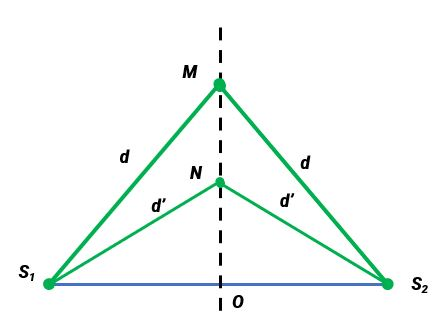
\includegraphics[scale=0.7]{../figs/VN12-PH-11-A-007-3-V2-1.JPG}
\end{center}

Điểm M nằm trên trung trực $\text{S}_1 \text{S}_2$ sẽ cách đều 2 nguồn một khoảng là $d$. Phương trình dao động của của 2 nguồn là
\begin{equation*}
	u_1=u_2=A \cos \omega  t.
\end{equation*}

Phương trình sóng truyền từ nguồn $\text{S}_1$ và $\text{S}_2$ đến M lần lượt là
\begin{eqnarray*}
	u_{\text{1M}}&=&A \cos \left(\omega  t - \dfrac{2\pi d}{\lambda} \right),\\
	u_{\text{2M}}&=&A \cos \left(\omega  t - \dfrac{2\pi d}{\lambda} \right).
\end{eqnarray*}

Phương trình dao động của M:
\begin{equation*}
	u_{\text{M}}= u_{\text{1M}}+u_{\text{2M}}=2A \cos \left(\omega  t - \dfrac{2\pi d}{\lambda} \right).
\end{equation*}

Nhận xét:

\begin{itemize}
	\item Điểm M dao động trễ pha so với hai nguồn
	\begin{equation*}
		\Delta \varphi =\dfrac{2\pi d}{\lambda}.
	\end{equation*}
	\item Điểm M lệch pha so với N là 
	\begin{equation*}
		\Delta \varphi' =\dfrac{2\pi (d-d')}{\lambda}.
	\end{equation*}
	\item Điểm M cùng pha với nguồn khi 
	\begin{equation*}
		\Delta \varphi=k2\pi\Leftrightarrow d=k\lambda.
	\end{equation*}
	\item Điểm M ngược pha với nguồn khi 
	\begin{equation*}
		\Delta \varphi=(2k+1)\pi\Leftrightarrow d=(k + \text{0,5})\lambda.
	\end{equation*}
	\item Điểm M vuông pha với nguồn khi
	\begin{equation*}
		\Delta \varphi=\left(k+\dfrac{1}{2}\right)\pi\Leftrightarrow  d=(k+ \text{0,5})\dfrac{\lambda}{2}.
	\end{equation*}
\end{itemize}
\subsection{Xác định điểm xa nhất hoặc gần nhất thỏa điều kiện về biên độ}
\subsubsection{Điểm nằm trên đường thẳng vuông góc đoạn nối hai nguồn}
Xét bài toán tìm trên đường thẳng $d$ vuông góc với 2 nguồn $\text{S}_1\text{S}_2$ tại $\text{S}_1$, điểm cực đại cách xa nhất và gần nhất với nguồn $\text{S}_1$ (hoặc tới đoạn thẳng nối 2 nguồn) khi 2 nguồn cùng pha.
\begin{center}
	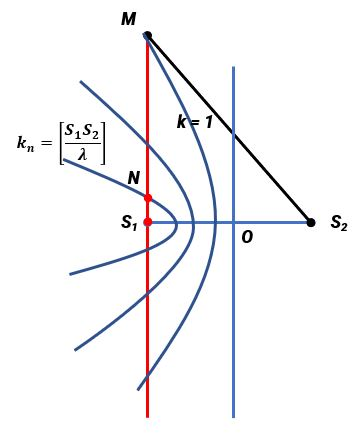
\includegraphics[scale=0.6]{../figs/VN12-PH-11-A-007-4-V2-1.JPG}
\end{center}
\begin{itemize}
	\item Điểm cực đại cách nguồn $\text{S}_1$ xa nhất khi nó nằm trên đường cực đại $k = 1$ (điểm M trên hình). Khi đó:
	\begin{equation*}
		\begin{cases}
			\text{MS}_2 - \text{MS}_1 =\lambda \\
			\text{MS}_2^2 - \text{MS}_1^2=\text{S}_1\text{S}_2^2
		\end{cases}.
	\end{equation*}
	
	
	\begin{equation*}
		\Rightarrow d_{\text{max}}=\text{MS}_1.
	\end{equation*}
	\item  Điểm cực đại cách nguồn $\text{S}_1$ gần nhất khi nó nằm trên đường cực đại ngoài cùng bậc $k_n$ (điểm N trên hình). Khi đó:
	\begin{equation*}
		\begin{cases}
			\text{NS}_2 - \text{NS}_1 =k_n\lambda \\
			\text{NS}_2^2 - \text{NS}_1^2=\text{S}_1\text{S}_2^2
		\end{cases}.
	\end{equation*}
	\begin{equation*}
		\Rightarrow d_{\text{min}}=\text{NS}_1.
	\end{equation*}
	Nếu $\dfrac{\text{S}_1\text{S}_2}{\lambda}$ không nguyên thì ta tìm nhanh $k_n$ là phần nguyên của phép chia  $\left[\dfrac{\text{S}_1\text{S}_2}{\lambda}\right]$.
\end{itemize}


\luuy{
	\begin{itemize}
		\item Đối với cực tiểu, điểm nằm xa nhất với nguồn khi nằm trên đường hyperbol với hệ số $k+1/2=\pm 1/2$.
		
		\item Khi 2 nguồn ngược pha, các công thức của điểm cực đại và cực tiểu sẽ hoán đổi cho nhau.
		
		\item Khi 2 nguồn lệch pha bất kỳ ta sử dụng điều kiện cực đại, cực tiểu trong trường hợp hai nguồn lệch pha để tìm vân cực đại, cực tiểu ngoài cùng.
	\end{itemize}
}
\subsubsection{Điểm nằm trên đường tròn, hình vuông, hình chữ nhật, $\ldots$}
Xét bài toán tìm trên đường tròn có tâm O là trung điểm của $\text{S}_1\text{S}_2$, đường kính $\text{S}_1\text{S}_2$, điểm cực đại cách xa nhất và gần nhất với nguồn $\text{S}_1$ (hoặc tới đoạn thẳng nối 2 nguồn) khi 2 nguồn cùng pha.
\begin{itemize}
	\item Điểm cực đại cách nguồn $\text{S}_1$ xa nhất khi nó nằm trên đường cực đại ngoài cùng bên phải. Khi đó:
	
	\begin{equation*}
		\begin{cases}
			\text{NS}_1 - \text{NS}_2 =k_{\text{n}}\lambda \\
			\text{NS}_1^2 - \text{NS}_2^2=\text{S}_1\text{S}_2^2
		\end{cases}
	\end{equation*}
	\begin{equation*}
		\Rightarrow d_{\text{max}}=\text{NS}_1.
	\end{equation*}
	
	\item Điểm cực đại cách nguồn $\text{S}_1$ gần nhất khi nó nằm trên đường cực đại ngoài cùng bên trái. Khi đó:
	
	\begin{equation*}
		\begin{cases}
			\text{MS}_2 - \text{MS}_1 =k_{\text{n}}\lambda \\
			\text{MS}_2^2 - \text{MS}_1^2=\text{S}_1\text{S}_2^2
		\end{cases}
	\end{equation*}
	
	\begin{equation*}
		\Rightarrow d_{\text{min}}=\text{MS}_1.
	\end{equation*}
	
	\item Nếu $\dfrac{\text{S}_1\text{S}_2}{\lambda}$ không nguyên thì ta tìm nhanh $k_{\text{n}} = \left[\dfrac{\text{S}_1\text{S}_2}{\lambda}\right]$ .
	
\end{itemize}
\luuy{
	\begin{itemize}
		\item Đối với cực tiểu, điểm nằm xa $\text{S}_1$ nhất là thuộc cực tiểu ngoài cùng bên phải, điểm gần $\text{S}_1$ nhất thuộc cực tiểu ngoài cùng bên trái.
		
		\item Khi 2 nguồn ngược pha, lệch pha ta cũng làm tương tự nhưng sử dụng điều kiện cực đại, cực tiểu cho trường hợp hai nguồn lệch pha bất kỳ.
		
		\item Đối các đường tròn không giống trường hợp trên hoặc các loại hình học khác ta dựa vào tính chất hình học và cách xác định số điểm cực đại, cực tiểu trên một đoạn để xác định được điểm cần tìm nằm ở đường hyperbol nào.
	\end{itemize}
}
\section{Mục tiêu bài học - Ví dụ minh họa}
\begin{dang}{Xác định được điểm thỏa mãn\\ điều kiện về pha trên đường trung trực của đoạn nối hai nguồn}
	\viduii{3}{Trên mặt thoáng của chất lỏng có hai nguồn kết hợp A và B cách nhau 20 cm với phương trình dao động: $u_1 =u_2 = \cos \omega t\ \text{cm}$. Bước sóng $\lambda = 8\ \text{cm}$. Biên độ sóng không đổi. Gọi M là một điểm trên đường trung trực của AB dao động cùng pha với các nguồn A, B và gần trung điểm H của AB nhất. Tính khoảng cách HM.
	}
	{
		\begin{center}
			\textbf{Hướng dẫn giải}
			
			\vspace*{1em}
			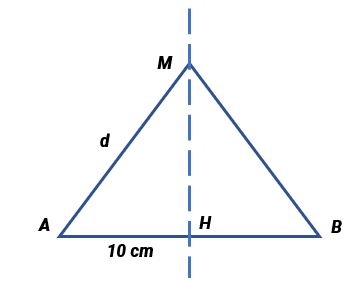
\includegraphics[scale=0.7]{../figs/VN12-PH-11-A-007-3-V2-2.JPG}
		\end{center}
		
		\begin{itemize}
			\item Điểm M nằm trên đường trung trực cách các nguồn một khoảng $d$ sẽ dao động cùng pha với các nguồn khi và chỉ khi $d=k\lambda$.
			\item Ta có $\text{AH} = 10\ \text{cm}, \lambda = 8\ \text{cm}$.
			\item Mà $d> \text{AH}$, suy ra:
			\begin{equation*} 
				8k >10 \Rightarrow k > \text{1,25}.
			\end{equation*}
			\item Điểm M gần H nhất nên $k$ là số nguyên nhỏ nhất. Suy ra $k=2$ và $d= 8 \cdot 2 =16\ \text{cm}$.
			\item Khoảng cách MH:
			\begin{equation*} 
				\text{MH}=\sqrt {16^2 -10^2} =2\sqrt {39} \ \text{cm}.
			\end{equation*}
		\end{itemize}
	}
	\viduii{4}
	{Hai nguồn phát sóng kết hợp $\text{S}_1, \text{S}_2$ trên mặt nước cách nhau 30 cm phát ra hai dao động điều hoà cùng phương, cùng tần số $f = 50\ \text{Hz}$ và pha ban đầu bằng 0. Biết tốc độ truyền sóng trên mặt chất lỏng $v = 6\ \text{m/s}$. Những điểm nằm trên đường trung trực của đoạn $\text{S}_1 \text{S}_2$ mà sóng tổng hợp tại đó luôn dao động ngược pha với sóng tổng hợp tại O (O là trung điểm của $\text{S}_1 \text{S}_2$) cách O một khoảng nhỏ nhất là
		
		\begin{mcq}(4)
			\item $5\sqrt 6\ \text{cm}$.
			\item $6\sqrt 6\ \text{cm}$.
			\item $4\sqrt 6\ \text{cm}$.
			\item $2\sqrt 6\ \text{cm}$.
		\end{mcq}
	}
	{\begin{center}
			\textbf{Hướng dẫn giải}
			
			\vspace*{1em}
			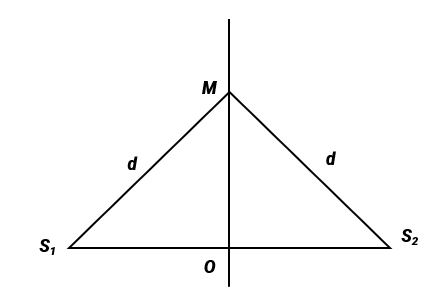
\includegraphics[scale=0.7]{../figs/VN12-PH-11-A-007-3-V2-3.JPG}
		\end{center}
		
		\begin{itemize}
			\item Giả sử hai sóng tại  $\text{S}_1$­,$\text{S}_1$ có dạng:
			\begin{equation*}
				u_1=u_2=a \cos \omega t.
			\end{equation*}
			\item  Gọi M là điểm thỏa mãn bài toán. Phương trình dao động tại M:
			\begin{equation*}
				u_{\text{M}} =2 a \cos \left(\omega t -\dfrac{2\pi d}{\lambda}\right).
			\end{equation*}
			\item Phương trình dao động tại O:
			\begin{equation*}
				u_{\text{O}} =2 a \cos \left(\omega t -\dfrac{2\pi \text{OS}_1}{\lambda}\right).
			\end{equation*}
			\item Độ lệch pha giữa M và O:
			\begin{equation*}
				\Delta \varphi = \varphi_{\text{M}} -\varphi_{\text{O}} = \dfrac{2\pi}{\lambda}(\text{OS}_1-d)=(2k+1) \pi \Rightarrow d = \text{OS}_1 - \dfrac{\lambda}{2}(2k+1)\ (*)
			\end{equation*}
			\item Mà $d>\text{OS}_1$ nên
			\begin{equation*}
				\text{OS}_1 - \dfrac{\lambda}{2}(2k+1) >\text{OS}_1 \Leftrightarrow 2k+1 <0 \Rightarrow  k < - \dfrac{1}{2}.
			\end{equation*}
			\item Từ biểu thức (*) ta thấy $d_{\text{min}}$ khi $k_{\text{max}} = -1$.
			\item Ta có:
			\begin{equation*}
				\text{OS}_1=\dfrac{\text{S}_1\text{S}_2}{2} =15\ \text{cm}.
			\end{equation*}
			\item Bước sóng $\lambda =\dfrac{v}{f} = 12\ \text{cm}$.
			\item Thay $k=-1$ vào (*) ta được $d =21\ \text{cm}$.
			\item Khoảng cách OM:
			\begin{equation*}
				\text{OM} =\sqrt{d^2-\text{OS}_1^2} = \sqrt{21^2-15^2}=\sqrt {216}=6\sqrt 6\ \text{cm}. 
			\end{equation*}
		\end{itemize}
		\textbf{Đáp án: B.}
	}
\end{dang}
\begin{dang}{Xác định được điểm gần nhất hoặc\\ xa nhất thỏa mãn điều kiện về biên độ trên đường thẳng vuông góc với đoạn nối hai nguồn}
	\viduii{3}
	{
		Tại mặt chất lỏng có hai nguồn phát sóng kết hợp $\text{S}_1$, $\text{S}_2$ cách nhau 16 cm, dao động điều hòa theo phương vuông góc với mặt chất lỏng với phương trình $u_1 = 2\cos 40\pi t\ \text{cm}$ và $u_2 = 2\cos40\pi t\ \text{cm}$. Tốc độ truyền sóng trên mặt chất lỏng là 40 cm/s. Gọi M là một điểm thuộc mặt chất lỏng, nằm trên đường thẳng $\text{S}_1$x vuông góc với $\text{S}_1\text{S}_2$, cách $\text{S}_1$ một đoạn ngắn nhất mà phần tử chất lỏng tại M dao động với biên độ cực tiểu. Khoảng cách M$\text{S}_1$ bằng
		\begin{mcq}(4)
			\item 1,425 cm.     
			\item 2,145 cm.     
			\item 2,075 cm.     
			\item 1,035 cm.
		\end{mcq}
	}
	{
		\begin{center}
			\textbf{Hướng dẫn giải}
			
			\vspace*{1em}
			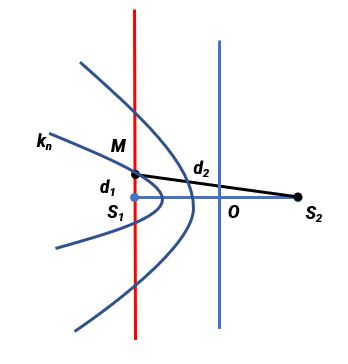
\includegraphics[scale=0.8]{../figs/VN12-PH-11-A-007-4-V2-2.JPG}
		\end{center}
		\begin{itemize}
			
			\item Bước sóng:
			$$\lambda = \dfrac{v}{f} = 2\ \text{cm}$$
			
			\item Số cực tiểu trên đoạn $\text{S}_1\text{S}_2$ được xác định như sau:
			
			\begin{equation*}
				-\dfrac{\text{S}_1\text{S}_2}{\lambda} -\dfrac{1}{2} < k < \dfrac{\text{S}_1\text{S}_2}{\lambda} - \dfrac{1}{2} \Rightarrow -\text{8,5}<k<\text{7,5}.
			\end{equation*}
			\item Suy ra $k=-8;...;-1;0;1...;7.$
			\item Để M cực đại và gần A nhất thì M phải nằm trên hypebol cực tiểu ngoài cùng ứng với $k_\text{n}=-8$.
			\item Vậy
			\begin{equation*}
				d_1-d_2=\left(-8+\dfrac{1}{2}\right) \lambda =-15.
			\end{equation*}
			\item Kết hợp với $d_2^2-d_1^2=\text{S}_1\text{S}_2^2 \Rightarrow d_2+d_1 = \dfrac{\text{S}_1\text{S}_2^2}{d_2-d_1}= \dfrac{16^2}{13} = \text{17,07}\ \text{cm}$.
			\item Suy ra $d_1=\text{1,035}\ \text{cm}$.
		\end{itemize}
		
		\textbf{Đáp án: D.}
	}
	\viduii{4}
	{
		Hai nguồn kết hợp A, B đồng bộ cách nhau 6 cm dao động, bước sóng 2 cm. Trên đường thẳng AC vuông góc với AB tại A, người ta thấy điểm M là cực đại nằm xa A nhất và nằm trên đường hyperbol ứng với giá trị $k$ ($k > 0$). Di chuyển nguồn B ra xa dọc theo đường thẳng nối hai nguồn ban đầu, khi đó điểm M tiếp tục nằm trên đường hyperbol cực tiểu thứ $k + 4$. Độ dịch chuyển nguồn B có thể là
		\begin{mcq}(4)
			\item 8 cm.    
			\item 9 cm.     
			\item 10 cm.    
			\item 12 cm.
		\end{mcq}
	}
	{
		\begin{center}
			\textbf{Hướng dẫn giải}
			
			\vspace*{1em}
			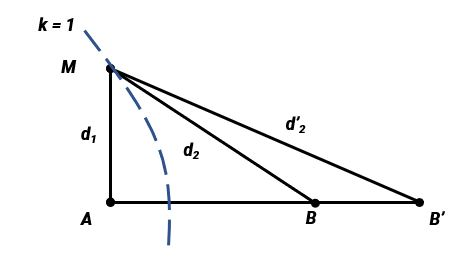
\includegraphics[scale=0.8]{../figs/VN12-PH-11-A-007-4-V2-3.JPG}
		\end{center}
		\begin{itemize}
			\item M là cực đại nằm xa A nhất, vậy M là cực đại ứng với $k = 1$.
			\item Ta có: 
			
			\begin{equation*}
				\begin{cases}
					d_2-d_1=\lambda = 2\ \text{cm}\\
					d_1^2+6^2=d_2^2
				\end{cases}
			\end{equation*}
			\begin{equation*}
				\Rightarrow d_1^2+6^2 = (d_1+2)^2.
			\end{equation*}
			\item Suy ra $d_1=8\ \text{cm}$.
			\item Dịch chuyển B đến B' thì M nằm trên cực tiểu thứ $k+4=5$
			\begin{equation*}
				\begin{cases}
					d'_2-d_1=\text{4,5}\lambda = 9\ \text{cm}\\
					d_2^{'2}=\text{AB}'^2+d_1^2.
				\end{cases}
			\end{equation*}
			\begin{equation*}
				\Rightarrow \text{AB}'=15\ \text{cm}. 
			\end{equation*}
			\item Suy ra $\text{BB}'=\text{AB}'-\text{AB}=15-6=9\ \text{cm}$.
		\end{itemize}
		
		\textbf{Đáp án: B.}
	}
\end{dang}
\begin{dang}{Xác định được điểm gần nhất hoặc\\ xa nhất thỏa mãn điều kiện về biên độ trên đường tròn, hình vuông,\\ hình chữ nhật, $\ldots$}
	\viduii{3}
	{Trong hiện tượng giao thoa sóng nước, hai nguồn dao động theo phương vuông góc với mặt nước, cùng biên độ, cùng pha, cùng tần số 50 Hz được đặt tại hai điểm $\text{S}_1$ và $\text{S}_2$ cách nhau 10 cm. Tốc độ truyền sóng trên mặt nước là 75 cm/s. Xét các điểm trên mặt nước thuộc đường tròn tâm $\text S_1$, bán kính $\text{S}_1\text{S}_2$, điểm mà phần tử tại đó dao động với biên độ cực đại cách điểm $\text{S}_2$ một đoạn ngắn nhất bằng
		\begin{mcq}(4)
			\item 85 mm.     
			\item 15 mm.    
			\item 10 mm.     
			\item 89 mm.
		\end{mcq}
	}
	{
		\begin{center}
			\textbf{Hướng dẫn giải}
			
			\vspace*{1em}
			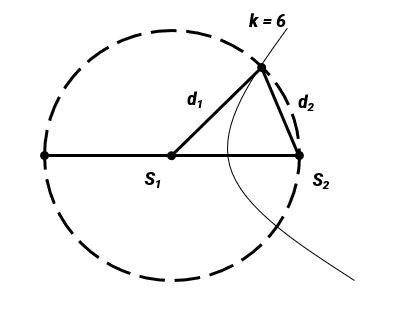
\includegraphics[scale=0.8]{../figs/VN12-PH-11-A-007-4-V2-4.JPG}
		\end{center}
		\begin{itemize}
			\item Bước sóng: 
			\begin{equation*}
				\lambda = \dfrac{v}{f}=\text{1,5}\ \text{cm}.
			\end{equation*}
			\item Số điểm dao động với biên độ cực đại trên $\text{S}_1\text{S}_2$:
			\begin{equation*}
				-\dfrac{\text{S}_1\text{S}_2}{\lambda} \leq k \leq \dfrac{\text{S}_1\text{S}_2}{\lambda} \Leftrightarrow -\text{6,6} \leq k \leq \text{6,6}.
			\end{equation*}
			
			\item Để điểm nằm trên đường tròn dao động cực đại và gần $\text{S}_2$ nhất thì điểm này phải thuộc hyperbol cực đại $k = 6$.
			
			\item Từ hình vẽ ta có: 
			\begin{equation*}
				d_1-d_2 = 6\lambda \Rightarrow  d_2 = d_1 - 6\lambda = \text{S}_1\text{S}_2 - 6\lambda = 1\ \text{cm}.
			\end{equation*}
			
		\end{itemize}
		
		\textbf{Đáp án: C.}
	}
	\viduii{3}
	{
		Trong hiện tượng giao thoa sóng hai nguồn kết hợp A, B cách nhau 20 cm dao động điều hòa cùng pha cùng tần số f = 40 Hz. Tốc độ truyền sóng trên mặt nước là 1,2 m/s. Xét trên đường tròn tâm A bán kính AB, điểm nằm trên đường tròn dao động với biên độ cực đại gần nhất, cách đường trung trực của AB khoảng bằng bao nhiêu?
		
		\begin{mcq}(4)
			\item 27,75 mm.     
			\item 26,1 mm.     
			\item 19,76 mm.     
			\item 32,4 mm.
		\end{mcq}
	}
	{
		\begin{center}
			\textbf{Hướng dẫn giải}
			
			\vspace*{1em}
			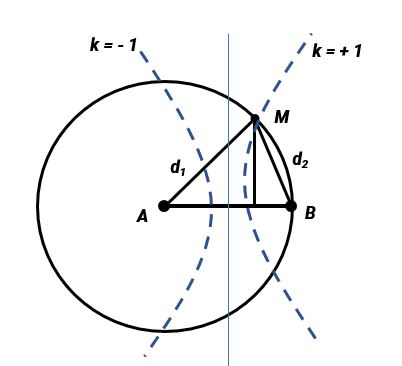
\includegraphics[scale=0.8]{../figs/VN12-PH-11-A-007-4-V2-5.JPG}
		\end{center}
		\begin{itemize}
			\item Bước sóng:
			\begin{equation*}
				\lambda = \dfrac{v}{f} = 3\ \text{cm}.
			\end{equation*}
			\item Số điểm dao động với biên độ cực đại trên AB:
			\begin{equation*}
				-\dfrac{\text{AB}}{\lambda} < k < \dfrac{\text{AB}}{\lambda} \Leftrightarrow -\text{6,6} \leq k \leq \text{6,6}.
			\end{equation*}
			\item Điểm nằm trên đường tròn dao động với biên độ cực đại và gần trung trực của AB nhất phải nằm trên các hyperbol cực đại ứng với $k = 1$ hoặc $k = -1$. Tuy nhiên trong trường hợp này ta thấy rằng điểm này phải nằm trên hyperbol $k = 1$.
			\item Suy ra $d_1 -d_2 =\lambda =3\ \text{cm} \Rightarrow d_2=d_1 - 3 =AB-3 =17\ \text{cm}$.
			\item Từ hình vẽ
			\begin{equation*}
				\begin{cases}
					d^2_2=h^2+x^2\\
					d^2_1=h^2 + (20-x)^2
				\end{cases}
			\end{equation*}
			\begin{equation*}
				\Rightarrow d_1^2-d_2^2 =(20-x)^2-x^2 \Rightarrow x =\text{7,225}\ \text{cm}.
			\end{equation*}
			\item Vậy khoảng cách này sẽ là $10-x=\text{2,775}\ \text{cm} =\text{27,75}\ \text{mm}$.
		\end{itemize}
		
		\textbf{Đáp án: A.}
	}
\end{dang}